\documentclass[9pt,]{book}
\usepackage[]{mathpazo}
\usepackage{amssymb,amsmath}
\usepackage{ifxetex,ifluatex}
\usepackage{fixltx2e} % provides \textsubscript
\ifnum 0\ifxetex 1\fi\ifluatex 1\fi=0 % if pdftex
  \usepackage[T1]{fontenc}
  \usepackage[utf8]{inputenc}
\else % if luatex or xelatex
  \ifxetex
    \usepackage{mathspec}
  \else
    \usepackage{fontspec}
  \fi
  \defaultfontfeatures{Ligatures=TeX,Scale=MatchLowercase}
\fi
% use upquote if available, for straight quotes in verbatim environments
\IfFileExists{upquote.sty}{\usepackage{upquote}}{}
% use microtype if available
\IfFileExists{microtype.sty}{%
\usepackage{microtype}
\UseMicrotypeSet[protrusion]{basicmath} % disable protrusion for tt fonts
}{}
\usepackage{hyperref}
\hypersetup{unicode=true,
            pdftitle={Supplement to Longitudinal analysis of child wasting and concurrence with stunting in low-resource settings},
            pdfauthor={Andrew Mertens et al.},
            pdfborder={0 0 0},
            breaklinks=true}
\urlstyle{same}  % don't use monospace font for urls
\usepackage{natbib}
\bibliographystyle{apalike}
\usepackage{longtable,booktabs}
\usepackage{graphicx,grffile}
\makeatletter
\def\maxwidth{\ifdim\Gin@nat@width>\linewidth\linewidth\else\Gin@nat@width\fi}
\def\maxheight{\ifdim\Gin@nat@height>\textheight\textheight\else\Gin@nat@height\fi}
\makeatother
% Scale images if necessary, so that they will not overflow the page
% margins by default, and it is still possible to overwrite the defaults
% using explicit options in \includegraphics[width, height, ...]{}
\setkeys{Gin}{width=\maxwidth,height=\maxheight,keepaspectratio}
\IfFileExists{parskip.sty}{%
\usepackage{parskip}
}{% else
\setlength{\parindent}{0pt}
\setlength{\parskip}{6pt plus 2pt minus 1pt}
}
\setlength{\emergencystretch}{3em}  % prevent overfull lines
\providecommand{\tightlist}{%
  \setlength{\itemsep}{0pt}\setlength{\parskip}{0pt}}
\setcounter{secnumdepth}{5}
% Redefines (sub)paragraphs to behave more like sections
\ifx\paragraph\undefined\else
\let\oldparagraph\paragraph
\renewcommand{\paragraph}[1]{\oldparagraph{#1}\mbox{}}
\fi
\ifx\subparagraph\undefined\else
\let\oldsubparagraph\subparagraph
\renewcommand{\subparagraph}[1]{\oldsubparagraph{#1}\mbox{}}
\fi

%%% Use protect on footnotes to avoid problems with footnotes in titles
\let\rmarkdownfootnote\footnote%
\def\footnote{\protect\rmarkdownfootnote}

%%% Change title format to be more compact
\usepackage{titling}

% Create subtitle command for use in maketitle
\providecommand{\subtitle}[1]{
  \posttitle{
    \begin{center}\large#1\end{center}
    }
}

\setlength{\droptitle}{-2em}

  \title{Supplement to Longitudinal analysis of child wasting and concurrence
with stunting in low-resource settings}
    \pretitle{\vspace{\droptitle}\centering\huge}
  \posttitle{\par}
    \author{Andrew Mertens et al.}
    \preauthor{\centering\large\emph}
  \postauthor{\par}
      \predate{\centering\large\emph}
  \postdate{\par}
    \date{2019-12-18}

\usepackage{booktabs}
\usepackage{amsthm}
\makeatletter
\def\thm@space@setup{%
  \thm@preskip=8pt plus 2pt minus 4pt
  \thm@postskip=\thm@preskip
}
\makeatother

\begin{document}
\maketitle

{
\setcounter{tocdepth}{1}
\tableofcontents
}
\chapter{Overview}\label{overview}

\textbf{Recommended citation:} Mertens A N, et al. 2020. Longitudinal
analysis of child wasting and concurrence with stunting in low-resource
settings. \emph{Journal Name}. doi.

This site contains supplementary information to the \emph{Longitudinal
analysis of child wasting and concurrence with stunting in low-resource
settings}.

\chapter{Sensitivity analysis using fixed effects}\label{fixed-effects}

\raggedright

The primary analyses presented in this manuscript pooled across
individual studies using random effects. Inferences about estimates from
fixed effects models are restricted to only the included
studies.\footnote{Hedges, L. V. \& Vevea, J. L. Fixed- and
  random-effects models in meta-analysis. Psychol. Methods 3, 486--504
  (1998).} The random effects approach is more conservative in the
presence of study heterogeneity and has larger confidence intervals
around each point estimate unless all cohort-specific estimates are very
similiar. Overall, the inference from results produced by each method
did not greatly differ.

\section{Age-specific prevalence}\label{age-specific-prevalence}

\subsection{Random effects}\label{random-effects}

\includegraphics[width=58.33in]{/Users/Nolan/Documents/Berkeley/Colford-Hubbard/ki/wasting/ki-longitudinal-manuscripts/figures/wasting/fig-wast-2-prev-overall_region--allage-primary}

\subsection{Fixed effects}\label{fixed-effects}

\includegraphics[width=58.33in]{/Users/Nolan/Documents/Berkeley/Colford-Hubbard/ki/wasting/ki-longitudinal-manuscripts/figures/wasting/fig-wast-2-prev-overall_region--allage-primary_FE}

\section{Age-specific incidence}\label{age-specific-incidence}

\subsection{Random effects}\label{random-effects-1}

\includegraphics[width=58.33in]{/Users/Nolan/Documents/Berkeley/Colford-Hubbard/ki/wasting/ki-longitudinal-manuscripts/figures/wasting/fig-wast-2-cuminc-overall_region--allage-primary}

\subsection{Fixed effects}\label{fixed-effects-1}

\includegraphics[width=58.33in]{/Users/Nolan/Documents/Berkeley/Colford-Hubbard/ki/wasting/ki-longitudinal-manuscripts/figures/wasting/fig-wast-2-cuminc-overall_region--allage-primary_FE}

\section{Age-specific incidence rate}\label{age-specific-incidence-rate}

\subsection{Random effects}\label{random-effects-2}

\includegraphics[width=58.33in]{/Users/Nolan/Documents/Berkeley/Colford-Hubbard/ki/wasting/ki-longitudinal-manuscripts/figures/wasting/fig-wast-2-ir-overall_region--allage-primary}

\subsection{Fixed effects}\label{fixed-effects-2}

\includegraphics[width=58.33in]{/Users/Nolan/Documents/Berkeley/Colford-Hubbard/ki/wasting/ki-longitudinal-manuscripts/figures/wasting/fig-wast-2-ir-overall_region--allage-primary_FE}

\section{Age-specific recovery}\label{age-specific-recovery}

\subsection{Random effects}\label{random-effects-3}

\includegraphics[width=58.33in]{/Users/Nolan/Documents/Berkeley/Colford-Hubbard/ki/wasting/ki-longitudinal-manuscripts/figures/wasting/fig-wast-2-rec-overall_region--allage-primary}

\subsection{Fixed effects}\label{fixed-effects-3}

\includegraphics[width=58.33in]{/Users/Nolan/Documents/Berkeley/Colford-Hubbard/ki/wasting/ki-longitudinal-manuscripts/figures/wasting/fig-wast-2-rec-overall_region--allage-primary_FE}

\section{Age-specific prevalence of severe
wasting}\label{age-specific-prevalence-of-severe-wasting}

\subsection{Random effects}\label{random-effects-4}

\includegraphics[width=58.33in]{/Users/Nolan/Documents/Berkeley/Colford-Hubbard/ki/wasting/ki-longitudinal-manuscripts/figures/wasting/fig-wast-3-prev-overall_region--allage-primary}

\subsection{Fixed effects}\label{fixed-effects-4}

\includegraphics[width=58.33in]{/Users/Nolan/Documents/Berkeley/Colford-Hubbard/ki/wasting/ki-longitudinal-manuscripts/figures/wasting/fig-wast-3-prev-overall_region--allage-primary_FE}

\section{Age-specific longitudinal prevalence of persistent
wasting}\label{age-specific-longitudinal-prevalence-of-persistent-wasting}

\subsection{Random effects}\label{random-effects-5}

\subsection{Fixed effects}\label{fixed-effects-5}

\includegraphics[width=25in]{/Users/Nolan/Documents/Berkeley/Colford-Hubbard/ki/wasting/ki-longitudinal-manuscripts/figures/wasting/fig-perswast_plot_FE}

\section{Age-specific prevalence of concurrent wasting and
stunting}\label{age-specific-prevalence-of-concurrent-wasting-and-stunting}

\subsection{Random effects}\label{random-effects-6}

\includegraphics[width=58.33in]{/Users/Nolan/Documents/Berkeley/Colford-Hubbard/ki/wasting/ki-longitudinal-manuscripts/figures/wasting/fig-wast-2-co-overall_region--allage-primary}

\subsection{Fixed effects}\label{fixed-effects-6}

\includegraphics[width=58.33in]{/Users/Nolan/Documents/Berkeley/Colford-Hubbard/ki/wasting/ki-longitudinal-manuscripts/figures/wasting/fig-wast-2-co-overall_region--allage-primary_FE}

\chapter{Cohort-specific estimates}\label{cohort}

\raggedright

Below are the cohort-specific estimates for the age-specific prevalences
of wasting, severe wasting, persistent wasting, underweight, and
concurrent wasting and stunting.

\section{Age-specific prevalence}\label{age-specific-prevalence-1}

\includegraphics[width=41.67in]{/Users/Nolan/Documents/Berkeley/Colford-Hubbard/ki/wasting/ki-longitudinal-manuscripts/figures/wasting/fig-prev_plot_africa}
\includegraphics[width=41.67in]{/Users/Nolan/Documents/Berkeley/Colford-Hubbard/ki/wasting/ki-longitudinal-manuscripts/figures/wasting/fig-prev_plot_lam}
\includegraphics[width=41.67in]{/Users/Nolan/Documents/Berkeley/Colford-Hubbard/ki/wasting/ki-longitudinal-manuscripts/figures/wasting/fig-prev_plot_sasia}

\section{Age-specific prevalence of severe
wasting}\label{age-specific-prevalence-of-severe-wasting-1}

\includegraphics[width=41.67in]{/Users/Nolan/Documents/Berkeley/Colford-Hubbard/ki/wasting/ki-longitudinal-manuscripts/figures/wasting/fig-sevwast_plot_africa}
\includegraphics[width=41.67in]{/Users/Nolan/Documents/Berkeley/Colford-Hubbard/ki/wasting/ki-longitudinal-manuscripts/figures/wasting/fig-sevwast_plot_lam}
\includegraphics[width=41.67in]{/Users/Nolan/Documents/Berkeley/Colford-Hubbard/ki/wasting/ki-longitudinal-manuscripts/figures/wasting/fig-sevwast_plot_sasia}

\section{Age-specific longitudinal prevalence of persistent
wasting}\label{age-specific-longitudinal-prevalence-of-persistent-wasting-1}

\includegraphics[width=41.67in]{/Users/Nolan/Documents/Berkeley/Colford-Hubbard/ki/wasting/ki-longitudinal-manuscripts/figures/wasting/fig-perswast_plot_africa}
\includegraphics[width=41.67in]{/Users/Nolan/Documents/Berkeley/Colford-Hubbard/ki/wasting/ki-longitudinal-manuscripts/figures/wasting/fig-perswast_plot_lam}
\includegraphics[width=41.67in]{/Users/Nolan/Documents/Berkeley/Colford-Hubbard/ki/wasting/ki-longitudinal-manuscripts/figures/wasting/fig-perswast_plot_sasia}

\section{Age-specific prevalence of concurrent wasting and
stunting}\label{age-specific-prevalence-of-concurrent-wasting-and-stunting-1}

\includegraphics[width=41.67in]{/Users/Nolan/Documents/Berkeley/Colford-Hubbard/ki/wasting/ki-longitudinal-manuscripts/figures/wasting/fig-co_plot_africa}
\includegraphics[width=41.67in]{/Users/Nolan/Documents/Berkeley/Colford-Hubbard/ki/wasting/ki-longitudinal-manuscripts/figures/wasting/fig-co_plot_lam}
\includegraphics[width=41.67in]{/Users/Nolan/Documents/Berkeley/Colford-Hubbard/ki/wasting/ki-longitudinal-manuscripts/figures/wasting/fig-co_plot_sasia}

\section{Age-specific prevalence of underweight (weight-for-age Z-score
\textless{}
-2)}\label{age-specific-prevalence-of-underweight-weight-for-age-z-score--2}

\includegraphics[width=41.67in]{/Users/Nolan/Documents/Berkeley/Colford-Hubbard/ki/wasting/ki-longitudinal-manuscripts/figures/wasting/fig-underweight_plot_africa}
\includegraphics[width=41.67in]{/Users/Nolan/Documents/Berkeley/Colford-Hubbard/ki/wasting/ki-longitudinal-manuscripts/figures/wasting/fig-underweight_plot_lam}
\includegraphics[width=41.67in]{/Users/Nolan/Documents/Berkeley/Colford-Hubbard/ki/wasting/ki-longitudinal-manuscripts/figures/wasting/fig-underweight_plot_sasia}

\chapter{Sensitivity analysis dropping at-Birth measures in
Kenaba}\label{no-kenaba}

\raggedright

Here, we re-estimate primary results after dropping the observations of
children at birth within the MRC Kenaba cohort, which used a different
team to measure child anthropometry at birth from the trained
anthropometrists used in follow-up measurements. While other cohort data
from the Kenaba area show that children tend to experience decreased LAZ
after birth, in the MRC Kenaba data used in this analysis, we see a high
birth LAZ (approximately 0) and a rapid drop in LAZ in followup
measurements (approximately -1 at one month). we see that the at birth
measurements LAZ is \textasciitilde{}0, and then for the follow-up
measurements after the mean LAZ is \textasciitilde{} -1 (and the mean
LAZ of just the subsequent follow-up visit at one month is
\textasciitilde{} -1). We calculated 30\% of measurements taken within
two weeks of birth are lower than the at birth measurement beyond the
technical error of measurement, and so are unrealistic decreases in
child length, and 43\% of follow-up measurements within two weeks of
birth are less than the at-birth measurement by any amount.

\section{Mean WLZ by region}\label{mean-wlz-by-region}

\includegraphics[width=41.67in]{/Users/Nolan/Documents/Berkeley/Colford-Hubbard/ki/wasting/ki-longitudinal-manuscripts/figures/wasting/WLZ_by_region-no-Kenaba-BW}

\section{Age-specific prevalence}\label{age-specific-prevalence-2}

\includegraphics[width=58.33in]{/Users/Nolan/Documents/Berkeley/Colford-Hubbard/ki/wasting/ki-longitudinal-manuscripts/figures/wasting/fig-wast-prev-no-Kenaba-BW}

\section{Age-specific incidence}\label{age-specific-incidence-1}

\includegraphics[width=58.33in]{/Users/Nolan/Documents/Berkeley/Colford-Hubbard/ki/wasting/ki-longitudinal-manuscripts/figures/wasting/fig-wast-ci-no-Kenaba-BW}

\section{Age-specific incidence
rate}\label{age-specific-incidence-rate-1}

\includegraphics[width=58.33in]{/Users/Nolan/Documents/Berkeley/Colford-Hubbard/ki/wasting/ki-longitudinal-manuscripts/figures/wasting/fig-wast-ir-no-Kenaba-BW}

\section{Age-specific recovery}\label{age-specific-recovery-1}

\includegraphics[width=58.33in]{/Users/Nolan/Documents/Berkeley/Colford-Hubbard/ki/wasting/ki-longitudinal-manuscripts/figures/wasting/fig-wast-rec-no-Kenaba-BW}

\section{Age-specific prevalence of severe
wasting}\label{age-specific-prevalence-of-severe-wasting-2}

\includegraphics[width=58.33in]{/Users/Nolan/Documents/Berkeley/Colford-Hubbard/ki/wasting/ki-longitudinal-manuscripts/figures/wasting/fig-sev-wast-no-Kenaba-BW}

\section{Age-specific longitudinal prevalence of persistent
wasting}\label{age-specific-longitudinal-prevalence-of-persistent-wasting-2}

\includegraphics[width=41.67in]{/Users/Nolan/Documents/Berkeley/Colford-Hubbard/ki/wasting/ki-longitudinal-manuscripts/figures/wasting/fig-pers-wast-no-Kenaba-BW}

\section{Age-specific prevalence of concurrent wasting and
stunting}\label{age-specific-prevalence-of-concurrent-wasting-and-stunting-2}

\includegraphics[width=58.33in]{/Users/Nolan/Documents/Berkeley/Colford-Hubbard/ki/wasting/ki-longitudinal-manuscripts/figures/wasting/fig-co-prev-no-Kenaba-BW}

\section{Age-specific prevalence of underweight (weight-for-age Z-score
\textless{}
-2)}\label{age-specific-prevalence-of-underweight-weight-for-age-z-score--2-1}

\includegraphics[width=58.33in]{/Users/Nolan/Documents/Berkeley/Colford-Hubbard/ki/wasting/ki-longitudinal-manuscripts/figures/wasting/fig-uw-prev-no-Kenaba-BW}

\chapter{Sensitivity analysis comparing wasting defined via
weight-for-length versus middle-upper arm circumference}\label{muac}

\raggedright

\includegraphics[width=58.33in]{/Users/Nolan/Documents/Berkeley/Colford-Hubbard/ki/wasting/ki-longitudinal-manuscripts/figures/wasting/fig-wast-2-muac-overall_region--allage-primary}

\chapter{Anthropometry measurement quality}\label{anthro}

\raggedright

\section{Anthropometry measuresments compared to WHO
standards}\label{anthropometry-measuresments-compared-to-who-standards}

To check for outliers in length measurements, We plotted the
distribution of raw length and weight measurements by age and sex
against bands marking the first, second, and third standard deviations
of the World Health Organization child growth standard distribution. The
majority of observations fell within 3 standard deviations of the mean
of the standard for males and females.

\includegraphics[width=33.33in]{/Users/Nolan/Documents/Berkeley/Colford-Hubbard/ki/wasting/ki-longitudinal-manuscripts/figures/shared/waz_QA_monthly}
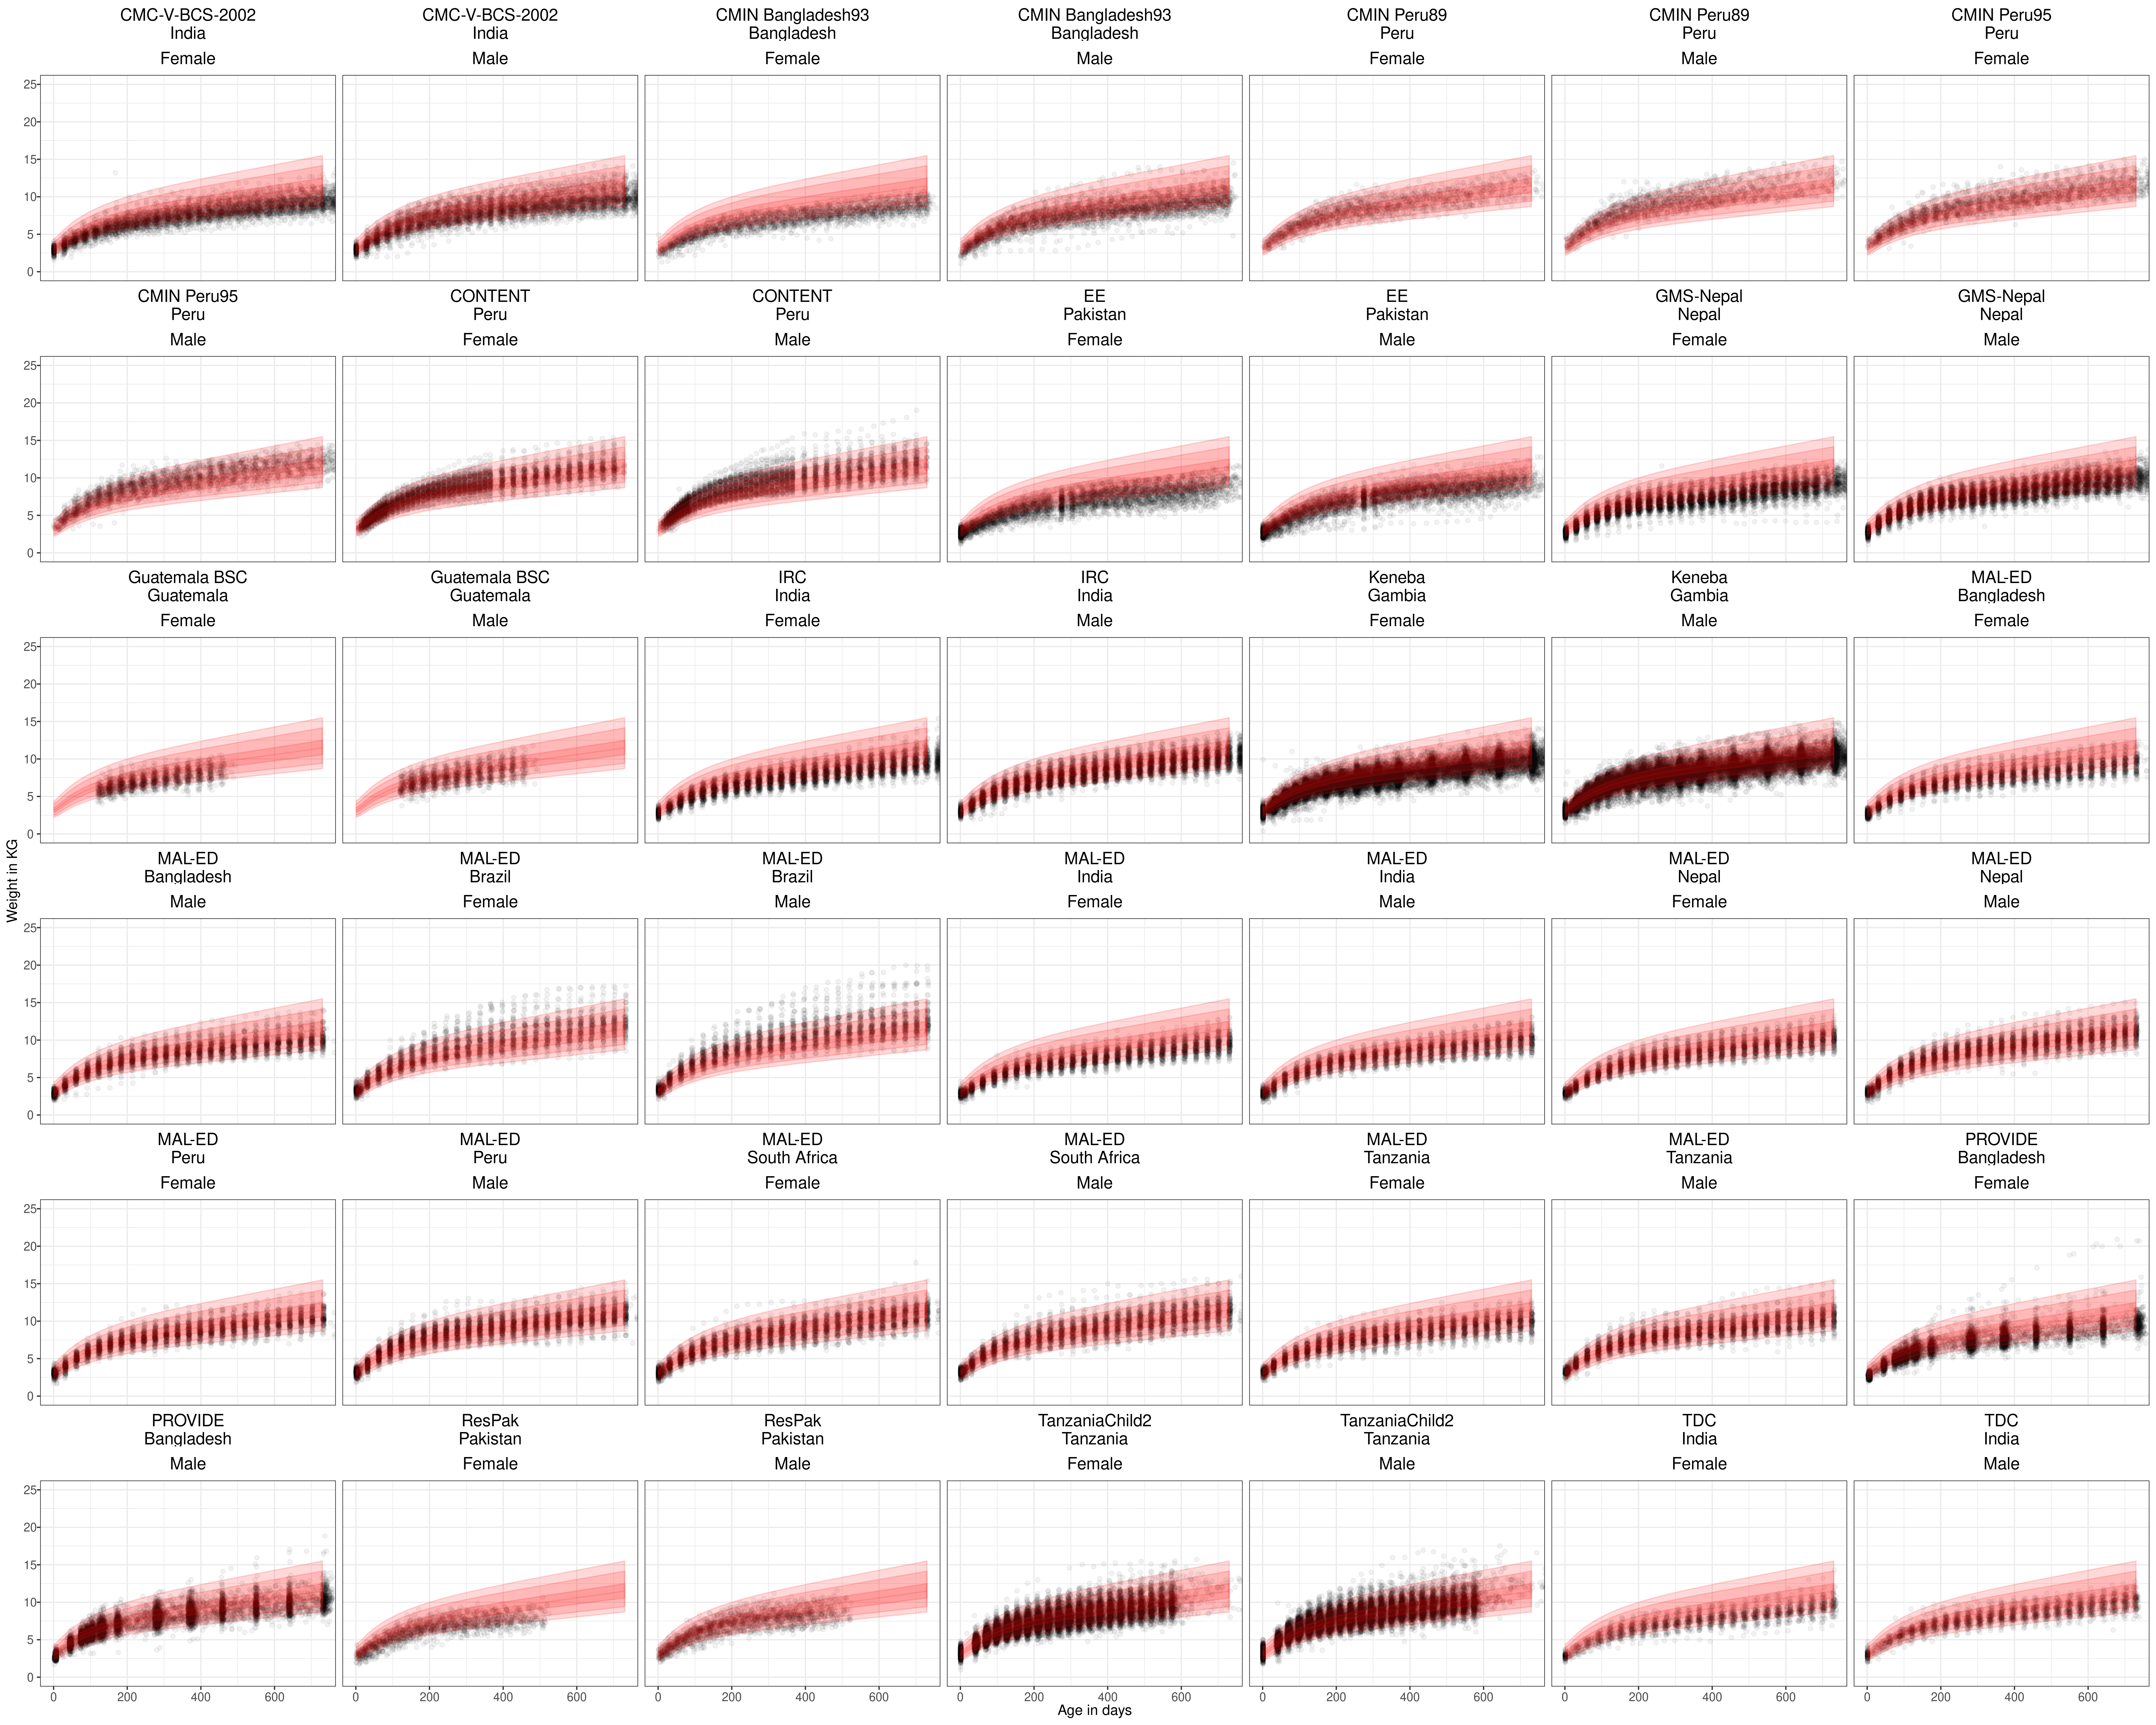
\includegraphics[width=104.17in]{/Users/Nolan/Documents/Berkeley/Colford-Hubbard/ki/wasting/ki-longitudinal-manuscripts/figures/shared/waz_QA_cohort_monthly}
\includegraphics[width=33.33in]{/Users/Nolan/Documents/Berkeley/Colford-Hubbard/ki/wasting/ki-longitudinal-manuscripts/figures/shared/laz_QA_monthly}
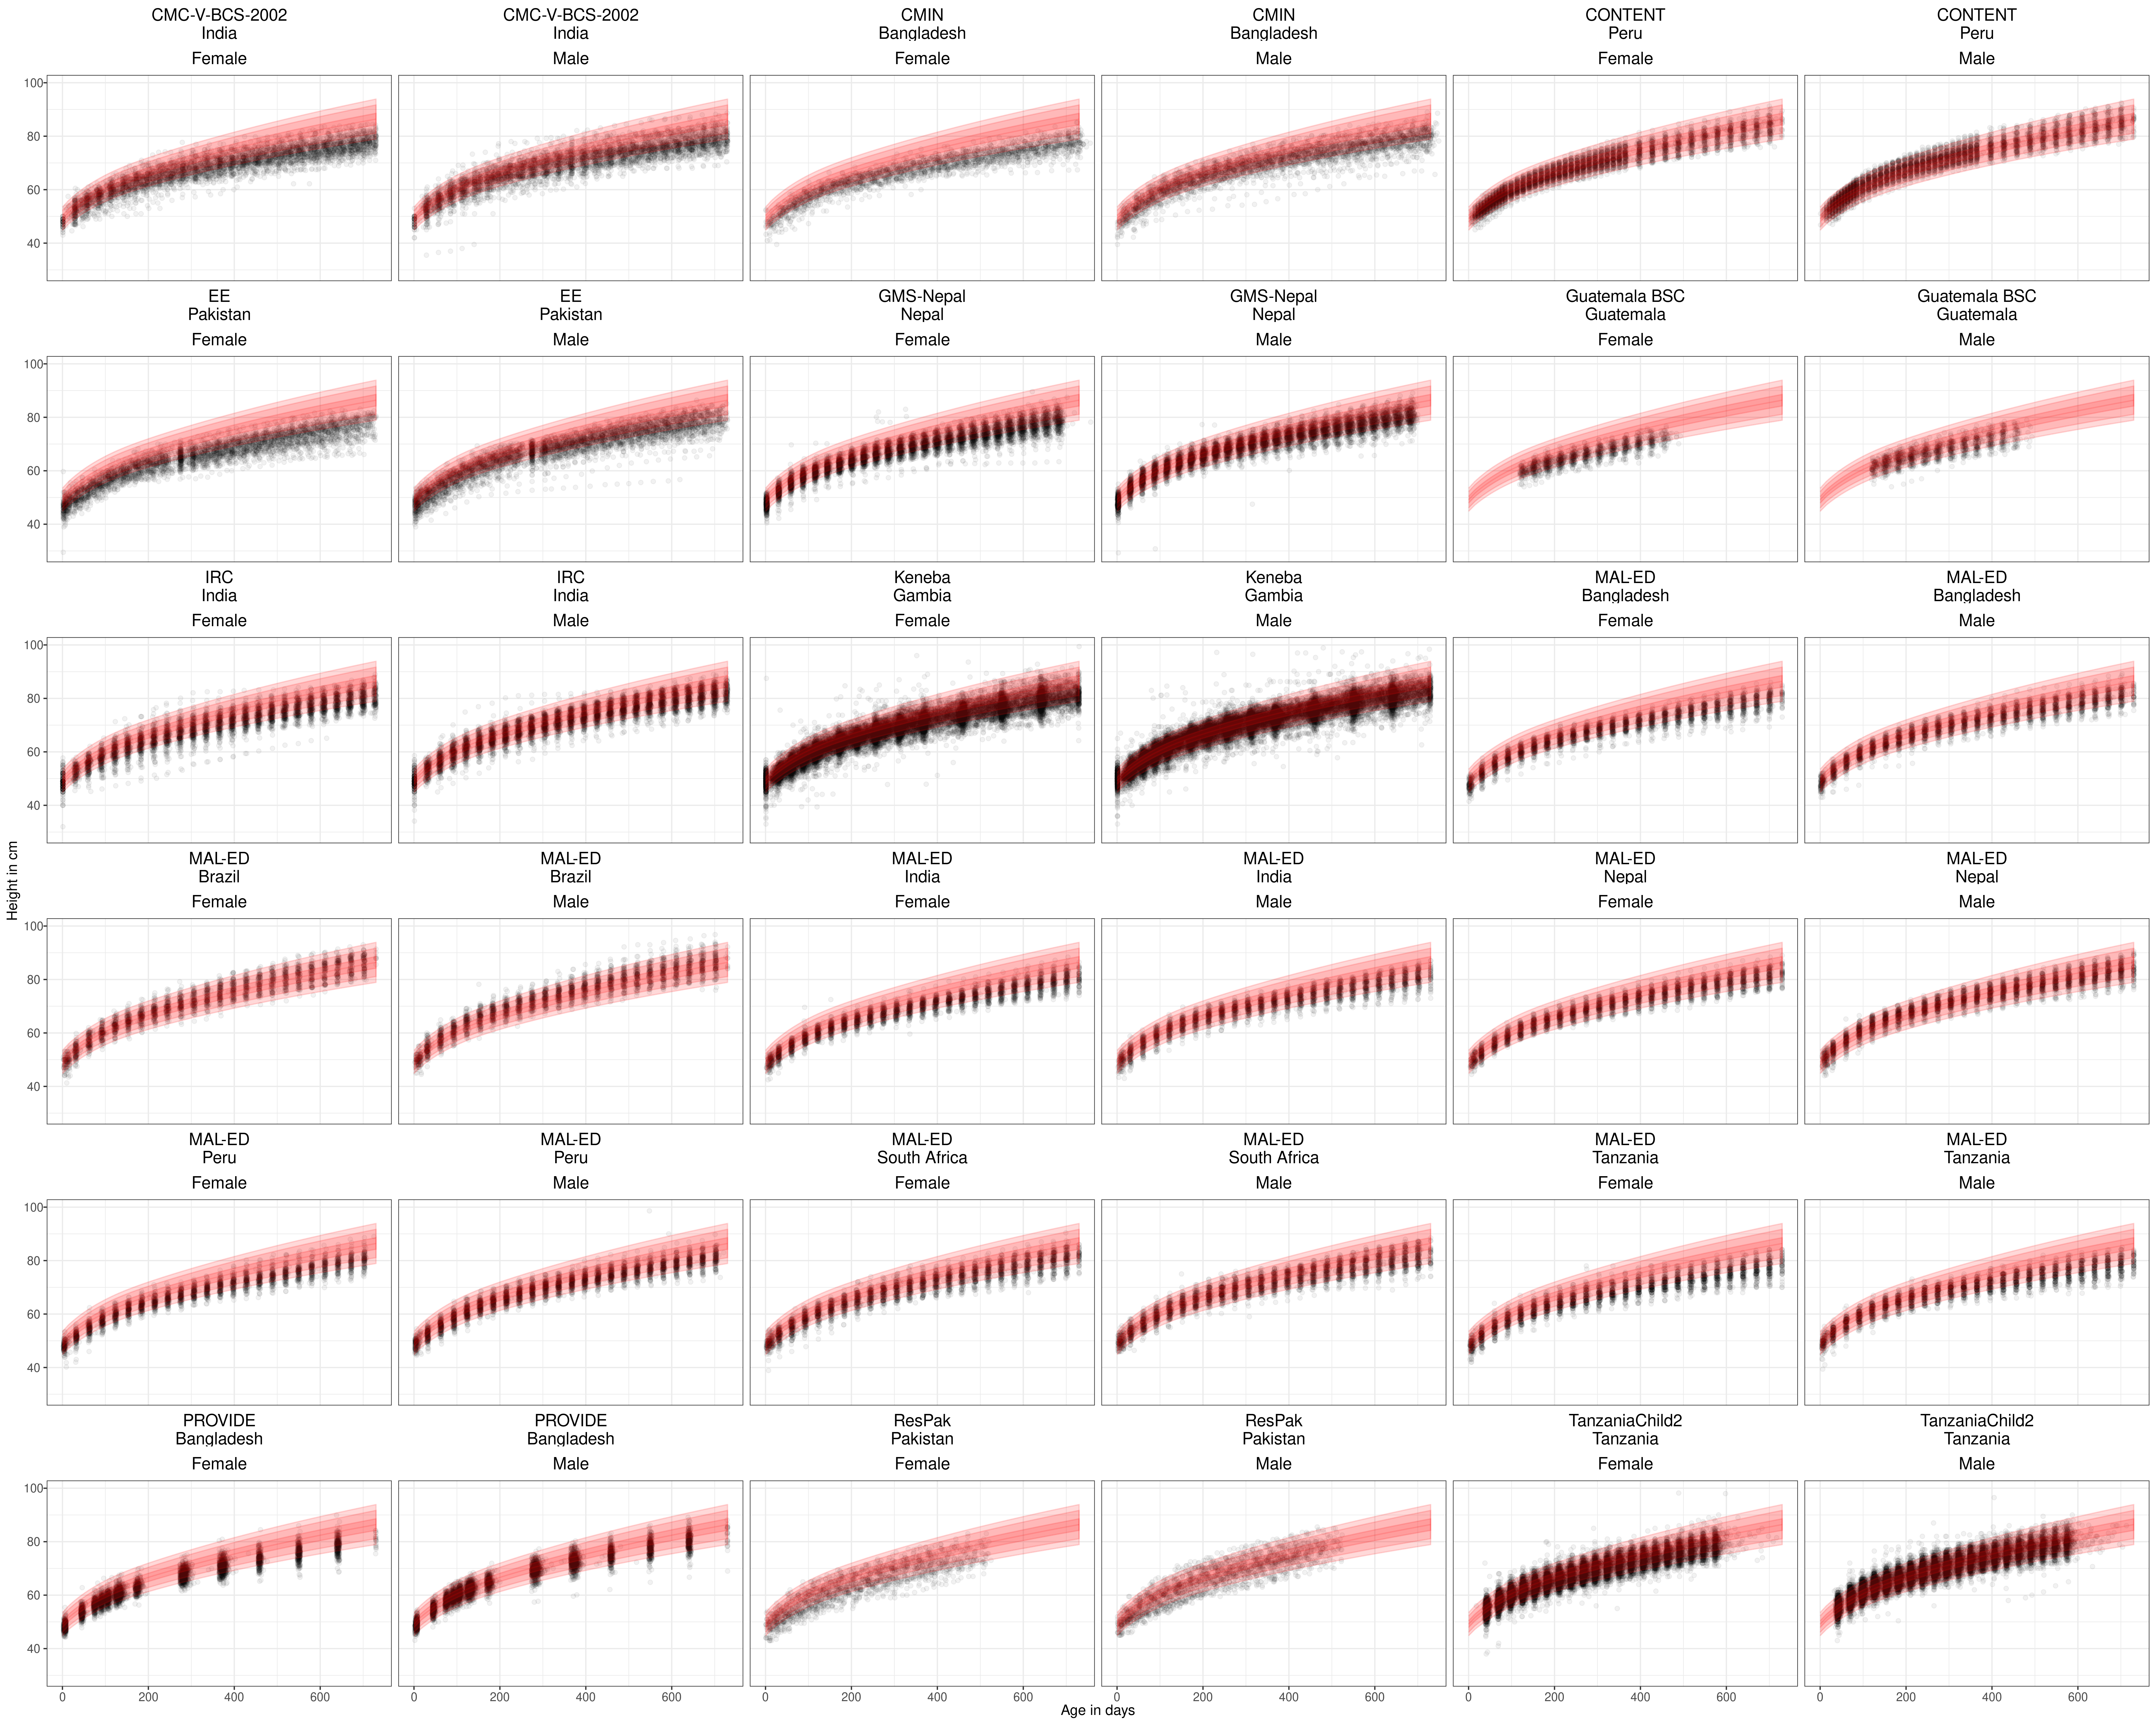
\includegraphics[width=104.17in]{/Users/Nolan/Documents/Berkeley/Colford-Hubbard/ki/wasting/ki-longitudinal-manuscripts/figures/shared/laz_QA_cohort_monthly}
\includegraphics[width=104.17in]{/Users/Nolan/Documents/Berkeley/Colford-Hubbard/ki/wasting/ki-longitudinal-manuscripts/figures/shared/wlz_QA_monthly}
\includegraphics[width=104.17in]{/Users/Nolan/Documents/Berkeley/Colford-Hubbard/ki/wasting/ki-longitudinal-manuscripts/figures/shared/wlz_QA_cohort_monthly}

\section{Age-specific incidence}\label{age-specific-incidence-2}

This study included cohorts that measured child growth from 1987 to
2014. To assess potential secular trends, we plotted the mean LAZ, WAZ,
and WLZ over time. The plot below shows the individual observations from
included studies over this range of years. There does not appear to be a
secular trend in LAZ, WAZ, or WLZ.

\includegraphics[width=33.33in]{/Users/Nolan/Documents/Berkeley/Colford-Hubbard/ki/wasting/ki-longitudinal-manuscripts/figures/shared/waz_secular_trend_monthly}
\includegraphics[width=33.33in]{/Users/Nolan/Documents/Berkeley/Colford-Hubbard/ki/wasting/ki-longitudinal-manuscripts/figures/shared/laz_secular_trend_monthly}
\includegraphics[width=33.33in]{/Users/Nolan/Documents/Berkeley/Colford-Hubbard/ki/wasting/ki-longitudinal-manuscripts/figures/shared/wlz_secular_trend_monthly}

\bibliography{book.bib,packages.bib}


\end{document}
